\chapter{Introduction}

\section{Background}\label{section:background}

\tb{The self-organisation of cells} into an apparent order appears across many different fields within biology. For example, the distribution of cells during the developmental process of an embryo, the growth of cancerous tissue \cite{morph}, vertebrate limb development \cite{miura1,glimm,miura2}, and pattern formation on animal coats (e.g spots on a jaguar \cite{painter}, feathers on birds \cite{bailleul}). Wolpert \cite{wolpert} presented the idea that, underpinning the development of shape and form (morphogenesis) is a cell's ability to differentiate according to its position in space and time. Furthermore, the concentration of certain chemicals (morphogens), or the concentration gradients of certain morphogens across a spatial domain of cells, affects the cell differentiation mechanism, and thus cells adopt a state relative to the concentration of a specific morphogen that they are exposed to.

The mechanism allowing cells to adopt an appropriate state is known as differential gene expression, and depends crucially on the communication between cells, achieved through cellular signalling \cite{gaffmonk}. Typical reaction-diffusion systems assume a negligible timescale on which the cellular signalling and gene expression processes occur. The gene expression process is however extremely complex and proceeds through several stages \cite{gaffmonk}, \tb{including} gene transcription and gene translation. These sub-processes can take large amounts of time, and it has been experimentally shown that these time delays are typically on the order of minutes, but in some cases can be as large as a few hours \cite{gaffmonk,tennyson}. These time delays can therefore be on the same order of magnitude as the pattern formation process itself. For example, the basic body plan of a zebrafish is established in less than 24 hours \cite{gaffmonk,kimmel}. It is therefore important to consider these delays when studying pattern formation in Turing mechanisms.

In 1952 \cite{turing}, Alan Turing proposed that the morphogenesis process could be mathematically modelled on a purely chemical basis via the interaction of morphogens, whose evolutions are described by a system of coupled reaction-diffusion equations. Turing showed that a stable steady state, robust to small perturbations in the spatially homogeneous setting (no diffusion), could become unstable and sensitive to small perturbations with the introduction of diffusion, leading to spatially inhomogeneous patterns. Cell fate decisions are then based on these morphogen concentrations, where regions of high morphogen or low morphogen concentration can lead to different cell fate decisions. Turing's model is therefore one of pre-patterning, where the morphogen pattern concentrations across a spatial domain are modelled, which in turn lead to cell fate decisions at a later stage. Typical reaction-diffusion systems in the context of Turing pattern formation consist of two partial differential equations, describing the interaction and evolution of two morphogens, the \textit{activator} and \textit{inhibitor}. Empirical evidence suggests that Turing instabilities are present in real biological systems, and can be used to explain complex biological phenomena \cite{yigaffneyli,molecular,miura,miura2,sick}. \tb{Whether Turing patterns can be recreated experimentally however with simple two-species systems is still very much an active field of research \cite{bespoke}.}

Time delays have been investigated in the context of Turing patterns, both numerically and analytically, through the incorporation of constant fixed time delays. One of the canonical reaction-diffusion mechanisms that exhibits Turing instabilities is the Schnakenberg model \cite{schnakenberg}. This model has been extensively studied in the context of Turing pattern formation with incorporated gene expression time delays. Two biologically motivated variants, the ligand-internalisation (LI) and reverse ligand-binding (RLB) models, have been considered in the literature. \tb{We briefly outline the biological motivation for these variants in \ref{section:fixedeq}}. The Schnakenberg reaction kinetics can be described as \textit{cross} kinetics \cite{leegaffney}, where the inhibitor upregulates the activator, which in turn downregulates the inhibitor. The LI model places gene expression time delay in purely the activator's dynamics, whereas the RLB model contains time delay in both the activator's and inhibitor's dynamics.

The numerical results in \cite{gaffmonk}, which studied the LI variant of the Schnakenberg model, showed that the time taken until pattern formation occurs drastically increases as the gene expression time delay in the model is increased, and that small delays, on the order of minutes, can cause a large increase in time-to-pattern, on the order of several hours, compared to a model with no time delay. This highlights the importance of studying gene expression time delays, especially when considering patterning events that occur on a fast timescale. The two papers \cite{jiang, yigaffneyli} consider both the LI and RLB variants of the Schnakenberg model. Using linear analysis and dynamical systems theory, the results in both suggest that the RLB model can exhibit spatially inhomogeneous temporal oscillations, as well as de-stabilisation of spatially inhomogeneous steady states, inhibiting pattern formation via Turing instabilities. The results in \cite{yigaffneyli}  specifically suggest that for the LI model in particular, extensive ligand internalisation, i.e increasing the time delay in the activator's dynamics, can antagonise the formation of patterns from Turing instabilities, shrinking the parameter space where Turing instabilities may occur. \tb{We expore these observations in more detail by conduction bifurcation analysis neglected in the analysis carried out in \cite{yigaffneyli}}.

Another typical reaction-diffusion system studied in \tb{the} literature is the Gierer-Meinhard (GM) model \cite{gm}. General results in both \cite{leegaffney,leegaffmonk} suggest that time delay causes a significant effect on the time taken until pattern formation occurs. Both papers also suggest that linear theory is insufficient in determining the presence of oscillations, and \cite{leegaffmonk} suggests that the severity of the effect that time delays will have on the timescales on which patterning events will occur cannot be accurately predicted from linear theory. A final observation from \cite{gaffmonk,leegaffmonk}, for both LI and RLB models, is that an increasing time delay may also increase the sensitivity of the final pattern formation to variation in initial conditions.

More recently analysis of one-dimensional spike solutions of the GM model in \cite{fadai1,fadai2}\footnote{We note that the spike solution analysis considered in \cite{fadai1,fadai2} differs from the linear stability of homogeneous steady states considered in \cite{leegaffmonk,gaffmonk,leegaffney}.}, show that the biological interpretation, and thus the placement of delay terms in the model, can affect the size of the parameter regimes for which the spike solution is linearly stable. It was found that, depending on the positioning of time-delayed terms, an increasing time delay can act as a stabilising or de-stabilising agent, enlarging or shrinking the stable parameter region of the spike. Further details of spike solutions of the GM model and their stability analysis can also be found in \cite{spike}. This analysis highlighted the importance of time delay positioning in the GM model for the stability of spike solutions. We aim to show an analogous result for the Turing space of the GM model, namely that altering the time-delayed terms within the model can change the effect that an increasing time delay has on the Turing space (the parameter regions such that Turing instabilities can occur).

Paradoxically, we see that although Turing's models can be used to explain and reproduce complex biological phenomena \cite{leegaffney}, the results seem to be dependent on gene expression dynamics, and as most of the current literature shows, gene expression time delays can provide difficulty in applying Turing's models to real systems. In summary, most of the literature shows that gene expression time delays increase the time-to-pattern, and that depending on the positioning of the time-delayed terms, an increasing time-delay can increase sensitivity of the final pattern formation to initial and boundary conditions, as well as shrink Turing spaces and antagonise pattern formation. The former effect in particular is an obstacle to using Turing mechanisms due to the timescales involved. Time delays can induce much larger delays in pattern onset, compared to the otherwise fast pattern onset that would occur without time delay, calling into question how relevant and applicable Turing's models are for patterning events on fast timescales.

We note that the current literature \tb{on Turing pattern formation in development} is only concerned with fixed time delays. On a cellular level however, the biological processes responsible for gene expression are inherently stochastic \cite{raj,elowitz,mcadams,paulsson}. Time delays, and more specifically distributed delays, have been motivated throughout mathematical biology. Distributed time delays have been incorporated to model biological phenomena such as hematopoiesis, and lactose operon dynamics \cite{newdist}, Wnt/$\beta$-catenin signalling pathways \cite{signal}, and Oncolytic virotherapy treatment for cancer \cite{cancer}. A distributed delay can be thought of as a more `general and realistic' \cite{cancer} approach to modelling, on a larger scale, a process which in reality may possess, on a small scale, an intrinsic stochasticity. Within the context of Turing pattern formation, introducing a fixed time delay into the reaction-diffusion mechanism is an oversimplification of the underlying biological process on a microscopic level, and leads us to consider a distribution of time delays at the macroscopic level \cite{bratsun,krausenew}.

In this dissertation we are interested in conducting a more systematic study of the time-to-pattern properties of models with fixed time delay, and a more careful consideration of sensitivity to initial and boundary conditions. We are also concerned with whether implementing a different form of delay, specifically distributed delay, can alleviate some of the problems caused by the fixed delay case. For the rest of this Chapter, we outline some of the mathematical preliminaries used throughout this dissertation, including an outline of Turing pattern theory, and the numerical methods we use. In Chapter 2, we study the LI variant of the Schnakenberg model, where time-delayed terms are considered only in the activator's dynamics. We use numerical simulations to systematically evaluate the robustness of results in the current literature to variations in initial and boundary conditions. Our results show that, although the type of pattern we see may be affected by these variations, the relationship between time delay and time until onset of patterning is robust. We also extend the current linear analysis presented in \tb{\cite{yigaffneyli}} and study the effect of fixed time delays on the Turing space, as well as considering in more depth the effects that time delay have on the time lag until onset of patterning. Chapter 3 will focus on the distributed delay model, where we aim to produce novel linear analysis and show that an incorporated distributed delay behaves almost identically to a fixed delay, and thus in a sense, the distributions we use do not matter. Finally, in Chapter 4, we introduce the GM model for pattern formation, and present initial findings showing the effect of a fixed time delay on the Turing space. Furthermore, we highlight the importance of the positioning of the time-delayed terms on the results seen, and thus the importance of understanding the biological processes that lead to gene expression time delays. Since the first three chapters of the dissertation are concerned only with the Schnakenberg model, this is the model we introduce first. The GM model is only considered in Chapter 4.

\section{Model Introduction}
\subsection{Without Time Delay}
The mathematical model we will consider for \tb{in Chapters 1-3} is the Schnakenberg model \cite{schnakenberg} -- one of the simplest `toy' models that exhibit some of the key behaviours that we are interested in, and a model that has also been studied extensively in the context of fixed time delays. The model describes the evolution and interaction between two reactants, $U$ and $V$. Only considering two reactants is a gross simplification of the underlying biological processes responsible for pattern formation, but it is still a non-trivial case that can admit Turing instabilities. In this dissertation, we restrict our investigation to one spatial domain. The chemical reaction describing the Schnakenberg kinetics \cite{baker} is given by
\begin{equation}\label{chem}
A\xrightleftharpoons[c_{-1}]{c_1} U,\quad B\xrightarrow{c_2} V,\quad 2U+V\xrightarrow{c_3} 3U,
\end{equation}
where the $c_i$ represent reaction rates. The quantities $A$ and $B$ are substances whose evolution is not considered, and we assume a constant supply. We use $u$, $v$, $a$, and $b$ to denote the concentrations of substances $U$, $V$, $A$ and $B$ respectively. Letting the reactants diffuse, and applying the law of mass action with a non-dimensionalisation \cite{murray}, yields the reaction-diffusion system
\begin{equation}\label{system}
    \begin{split}
    \frac{\partial u}{\partial t}&=\frac{\epsilon^2}{L^2}\frac{\partial^2 u}{\partial x^2}+a-u+u^2v,\\
    \frac{\partial v}{\partial t}&=\frac{1}{L^2}\frac{\partial^2 v}{\partial x^2}+b-u^2v,
    \end{split}
\end{equation}
where $x\in\Omega=[0,1]$ is the non-dimensionalised spatial domain and $a,b>0$ are fixed parameters. The parameter $\epsilon^2$ can be thought of as the ratio of diffusion coefficients between the activator $u$ and inhibitor $v$, and $L^2$ a scaling of the domain length on which the problem is being solved. Typical values in the literature \cite{gaffmonk} are $L^2=1/200$ and $\epsilon^2=0.001$. Unless otherwise stated, in this dissertation we use the same $\epsilon^2=0.001$, and a domain size, $L$, $30$ times of that used in \cite{gaffmonk}, namely $L^2=9/2$. Since we are interested in the pattern formation arising from the self-organisation of cells, we implement no flux (homogeneous Neumann) boundary conditions on the boundary of the spatial domain, namely
\begin{equation}\label{neumannbc}
    \frac{\partial u}{\partial x}=\frac{\partial v}{\partial x}=0, \quad \quad x=0,1.
\end{equation}
As typical when studying Turing patterns, initial conditions $(u_0,v_0)$ are chosen as a small random Gaussian perturbation from the spatially homogeneous steady state $(u_\star,v_\star)$. In this dissertation, unless otherwise stated, the initial conditions we use are
\begin{equation}\label{firstic}
\begin{pmatrix}u_0\\v_0\end{pmatrix}=\begin{pmatrix}u_\star(1+r)\\v_\star(1+r)\end{pmatrix},
\end{equation}
where $r$ is a random variable such that $r\sim\mathcal{N}\left(0,0.01^2\right)$. The notation $r\sim\mathcal{N}\left(\mu_{\text{IC}},\sigma_{\text{IC}}^2\right)$ denotes a Normally distributed random variable $r$ with mean $\mu_{\text{IC}}$ and standard deviation of the initial perturbation $\sigma_{\text{IC}}$.

\subsection{With Fixed Time Delay}\label{section:fixedeq}

The form of the model we consider with fixed time delay is the LI variant of the standard Schnakenberg model. We do not consider the RLB model as it was found in \cite{william}, that under certain conditions, the numerical solutions of activator and inhibitor concentrations became physically infeasible, with negative solutions. The LI model assumes that a reaction at the cell surface is followed by internalisation of a morphogen before the gene expression process can continue and morphogen production can occur \cite{leegaffney,yigaffneyli}, introducing a time delay in the activator's dynamics.  This is based on the assumption that the gene expression process, and thus the source of the time delay, is responsible for autocatalysis of the activator in the reaction-diffusion mechanism \cite{gaffmonk}. As described in \cite{baker}, applying the delay to the final nonlinear term of \eqref{chem} yields the reaction described by
\begin{equation}\label{chem2}
A\xrightleftharpoons[c_{-1}]{c_1} U,\quad B\xrightarrow{c_2} V,\quad 2U+V\xrightarrow{c_3} W,\quad W\xrightarrow{\text{\footnotesize delay } \tau}3U.
\end{equation}
The reaction describes an internalisation of two particles of $U$, and one particle of $V$, which are removed from the reaction, forming substance $W$. However, three particles of $U$ are obtained from a reaction at a time $\tau$ in the past. The reaction-diffusion system describing the LI model is thus written as \cite{leegaffney}
\begin{equation}\label{fixed}
  \begin{split}
  \frac{\partial u}{\partial t}&=\frac{\epsilon^2}{L^2}\frac{\partial^2u}{\partial x^2}+a-u-2u^2v+3\hat{u}^2\hat{v},\\
  \frac{\partial v}{\partial t}&=\frac{1}{L^2}\frac{\partial^2v}{\partial x^2}+b-u^2v,
\end{split}
\end{equation}
where $u=u(x,t)$, $v=v(x,t)$ and $\hat{u}$, $\hat{v}$ are evaluated at some delay $\tau$, so that $\hat{u}=u(x,t-\tau)$ and $\hat{v}=v(x,t-\tau)$.

In order to solve delay differential equations (DDEs), a history function is required to define the solution for $t\in[-\tau,0)$ for the terms with time delay, so that the solutions of $u(x,t-\tau)$ and $v(x,t-\tau)$ are defined for $t\in[0,\tau)$. Throughout this dissertation, unless otherwise stated, a constant history function equal to the initial conditions is used, so that
\begin{equation}\label{hist}
    \begin{split}
u(x,t-\tau)&=u_0,\\
v(x,t-\tau)&=v_0,
\end{split}
\end{equation}
for all $x\in[0, 1]$ and $t\in[0,\tau]$.

\subsection{With Distributed Time Delay}

The stochastic nature of gene expression delays leads us to consider a mean-field approach to modelling the time delay \cite{bratsun,krausenew}. We can thus write the LI model with distributed time delay as

\begin{equation}\label{distmodel}
  \begin{split}
    \frac{\partial u}{\partial t}&=\frac{\epsilon^2}{L^2}\frac{\partial^2u}{\partial x^2}+a-u-2u^2v+3\int_{a}^{b}k(s;\textbf{p})\hat{u}^2\hat{v} \ \text{ds},\\
    \frac{\partial v}{\partial t}&=\frac{1}{L^2}\frac{\partial^2v}{\partial x^2}+b-u^2v,
\end{split}
\end{equation}
where $\hat{u}=u(x,t-s)$ and $\hat{v}=v(x,t-s)$, with $s$ the integration variable ranging over the delays. The function $k(s;\textbf{p})$ denotes some probability distribution function, with $s$ the integration variable, and $\textbf{p}$ the distribution parameters. The integration domain of delays is given by $[a,b]$ with $a>0$ to ensure positive time delays. Choices of different probability density functions will be considered in more detail in Chapter \ref{section:distdel}.

\section{Mathematical Preliminaries}
\subsection{Turing Pattern Formation Without Delay}
Here we give a brief overview of the mathematical theory underpinning Turing pattern formation, closely following the description in \cite{murray}. For further details, the reader should consult \cite{murray,beentjes}. Turing instabilities occur when the spatially homogeneous stable steady state becomes unstable in the presence of diffusion. We therefore first consider the spatially homogeneous model (the system defined in \eqref{system} without diffusive terms), and explore conditions necessary for the steady state to be stable. In the case of the Schnakenberg model, the single steady state occurs at $(u_\star, v_\star)=\left(a+b, \frac{b}{(a+b)^2}\right)$, with $u_\star,v_\star>0$. Following the methodology in \cite{murray}, we perform linear stability analysis. Taking a small perturbation from the steady state, so that $u(x,t)=u_\star+\delta\xi(x,t) $, $v(x,t)=v_\star+\delta\eta(x,t) $ for $|\delta|\ll1$, we consider the evolution of the perturbation. Denoting $\pmb{\xi}=\begin{bmatrix}\xi \\ \eta\end{bmatrix}$ as the vector of perturbations, and Taylor expanding up to $O(\delta)$, the linearised system of \eqref{system} is given as

\begin{equation}\label{linsys}
\frac{d\pmb{\xi}}{dt}=\textbf{J}_{(u_\star,v_\star)}\pmb{\xi},
\end{equation}
where $\textbf{J}_{(u_\star,v_\star)}$ is the Jacobian matrix of the kinetic equations evaluated at the steady state, namely,
$$
\textbf{J}_{(u_\star,v_\star)}=\begin{pmatrix}f_u&f_v\\g_u&g_v\end{pmatrix}\Bigg|_{(u_\star,v_\star)}.
$$
The notation $f_u$ is used to denote the partial derivative of $f$ with respect to $u$. For the Schnakenberg model (without time delay), the kinetic functions are given as
\begin{align*}
f(u,v)&=a-u+u^2v,\\
g(u,v)&=b-u^2v.
\end{align*}
\tb{We consider that} solutions of \eqref{linsys} are of the form
$$
\pmb{\xi}\propto e^{\lambda t},
$$
for eigenvalues $\lambda$ of $\textbf{J}_{(u_\star,v_\star)}$. The steady state is said to be asymptotically stable if the perturbation decays.
Denoting $\text{spec}(\textbf{M})$ as the set of eigenvalues of some matrix $\textbf{M}$, asymptotic stability occurs when $\Re(\lambda)<0 \ \text{for all }\lambda\in \text{spec}(\textbf{J}_{(u_\star,v_\star)})$. However, if there exists $\lambda\in \text{spec}(\textbf{J}_{(u_\star,v_\star)})\text{ such that } \Re(\lambda)>0$,
then the perturbation will grow with time and the steady state is unstable. The sum and product of the eigenvalues of $\textbf{J}_{(u_\star,v_\star)}$
are given by $\text{Tr}(\textbf{J}_{(u_\star,v_\star)})$ and $\text{det}(\textbf{J}_{(u_\star,v_\star)})$ respectively. The required conditions for stability are therefore
\begin{equation}\label{cond1}
    \begin{split}
\text{Tr}(\textbf{J}_{(u_\star,v_\star)})<0 &\implies (f_u+g_v)\big|_{(u_\star,v_\star)}<0, \\
\text{det}(\textbf{J}_{(u_\star,v_\star)})>0 &\implies (f_ug_v-f_vg_u)\big|_{(u_\star,v_\star)}>0.
\end{split}
\end{equation}

We now consider the full diffusive model and look for necessary conditions such that the previously stable steady state is driven to instability. The linearised system is given by
\begin{equation}\label{linsys2}
    \frac{\partial \pmb{\xi}}{\partial t}=\left[\textbf{D}\frac{\partial}{\partial x^2}+\textbf{J}_{(u_\star,v_\star)} \right]\pmb{\xi},
\end{equation}
where $\textbf{D}=\begin{pmatrix}\frac{\epsilon^2}{L^2}&0\\0&\frac{1}{L^2}\end{pmatrix}$ is the matrix containing the diffusion coefficients of reactants. The solution to the spatially dependent eigenvalue problem can be written as a linear combination of the eigenfunctions $w_k$ that satisfy the problem
\begin{equation}\label{eigprob}
\nabla^2w_k=-k^2w_k,\quad \quad \frac{\partial w_k}{\partial x}=0\quad x=0, 1.
\end{equation}
Considering only a regular 1D domain $\Omega=[0,1]$ with no flux boundary conditions, we note that the eigenfunctions will be of the form $w_k=\cos(k\pi x)$, $x\in[0,1]$. We thus look for solutions to \eqref{linsys2} of the form
\begin{equation}\label{perturbgrow}
    \pmb{\xi}=\sum_{k=0}^{\infty} \textbf{c}_ke^{\lambda_k t}w_k(x),
\end{equation}
where the constants $\textbf{c}_k$ are determined by using a Fourier expansion of the initial conditions in terms of the eigenfunctions $w_k$. $\lambda_k$ is the eigenvalue which determines the rate of temporal growth for each mode $k$, and thus determines whether a particular mode of pattern will be unstable and grow. Substituting this form \eqref{perturbgrow} into \eqref{linsys2}, along with using \eqref{eigprob} and simplifying, we obtain, for each $k$ \tb{by orthogonality}
$$
\lambda_k w_k=\textbf{J}w_k-\textbf{D}k^2w_k \implies (\lambda_k \textbf{I}-\textbf{J}+k^2\textbf{D})w_k=\textbf{0},
$$
with $\textbf{I}$ the identity matrix. Looking for non-trivial solutions for $w_k$, we solve for roots of the characteristic polynomial, namely $\text{det}(\lambda_k \textbf{I}-\textbf{J}+k^2\textbf{D})=0$, which yields a quadratic equation for eigenvalues $\lambda_k(k)$ as a function of $k$. Finding roots of this quadratic such that $\Re(\lambda_k(k))>0$ for some $k\neq0$, we conclude \cite{murray} two necessary conditions for the instability of the steady state in the presence of diffusion, namely
\begin{equation}\label{cond2}
    \begin{split}
    \left(\frac{1}{\epsilon^2}f_u+g_v\right)\bigg|_{(u_\star,v_\star)}>0,&\\
    \left(\left(\frac{1}{\epsilon^2}f_u+g_v\right)^2-\frac{4}{\epsilon^2}(f_ug_v-f_vg_u)\right)\bigg|_{(u_\star,v_\star)}>0.
\end{split}
\end{equation}
We therefore have four necessary conditions in terms of $(a,b,\epsilon^2)$ for Turing patterns to occur. These conditions are only necessary, and not sufficient, because conditions \eqref{cond2} assume $k$ to be a continuous variable, rather than discrete, and this is only strictly valid in the limit $L\to\infty$. Using the first two conditions in \eqref{cond1}, a bifurcation diagram in the $(a,b)$ parameter space can be plotted showing the regions corresponding to a stable or unstable steady state. This can be seen in Figure \ref{fig:bifsh}. Using the additional conditions in \eqref{cond2} and the fixed value $\epsilon^2=0.001$, the parameter region in the $(a,b)$ parameter space in which Turing patterns can occur can also be plotted. This `Turing space' can be seen in Figure \ref{fig:turingspace}. We note that throughout this dissertation, where results are presented for varying parameter values $(a,b)$, the parameter space is discretised at regular intervals of $0.02$, for both $a$ and $b$.

\begin{figure}[H]
    \centering
    \begin{subfigure}[t]{0.45\textwidth}
        \centering
        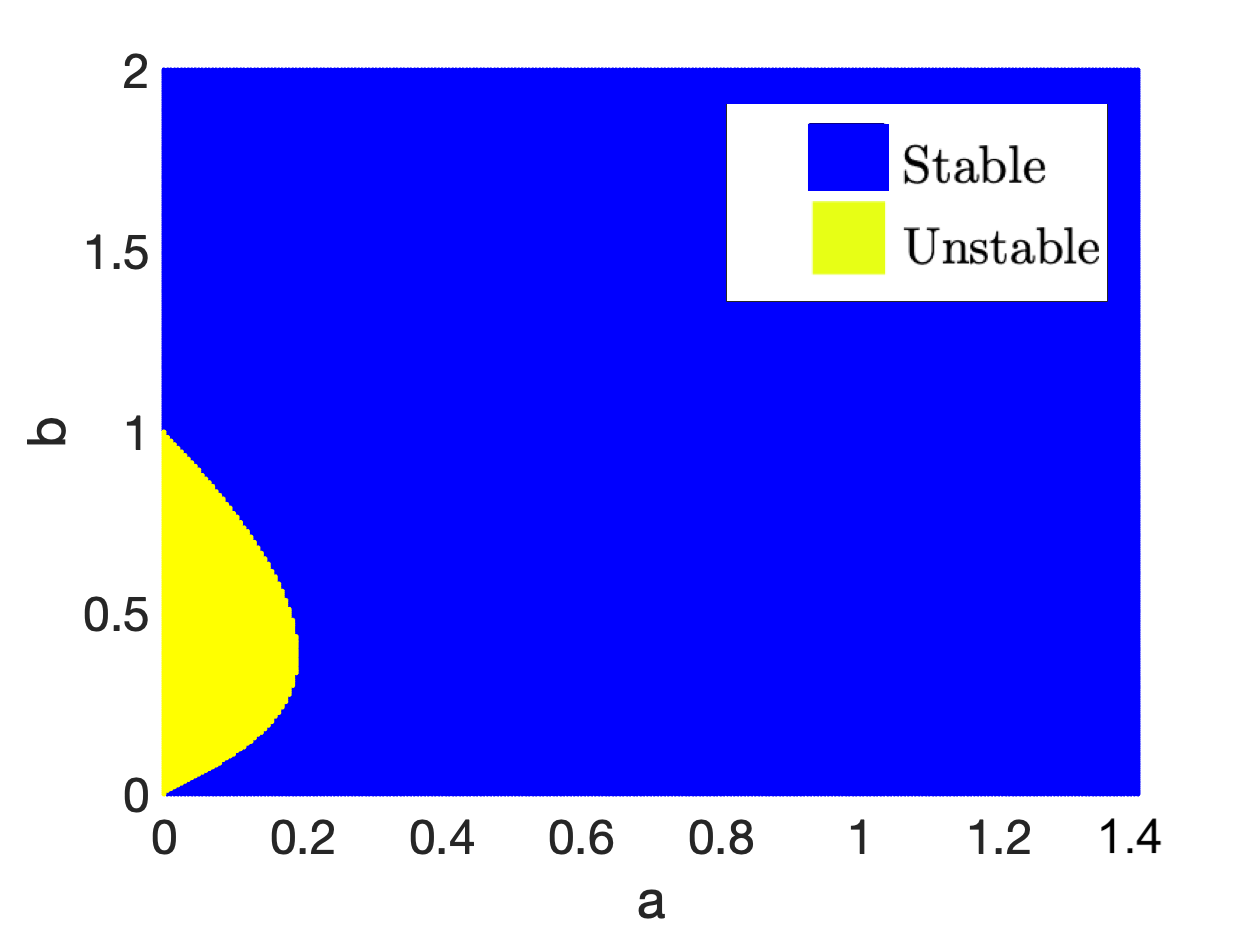
\includegraphics[width=7cm,height = 6cm]{bifsh1.png}
        \caption{Bifurcation diagram for spatially homogeneous model, no delay.}
        \label{fig:bifsh}
    \end{subfigure}
    \hfill
    \begin{subfigure}[t]{0.45\textwidth}
        \centering
        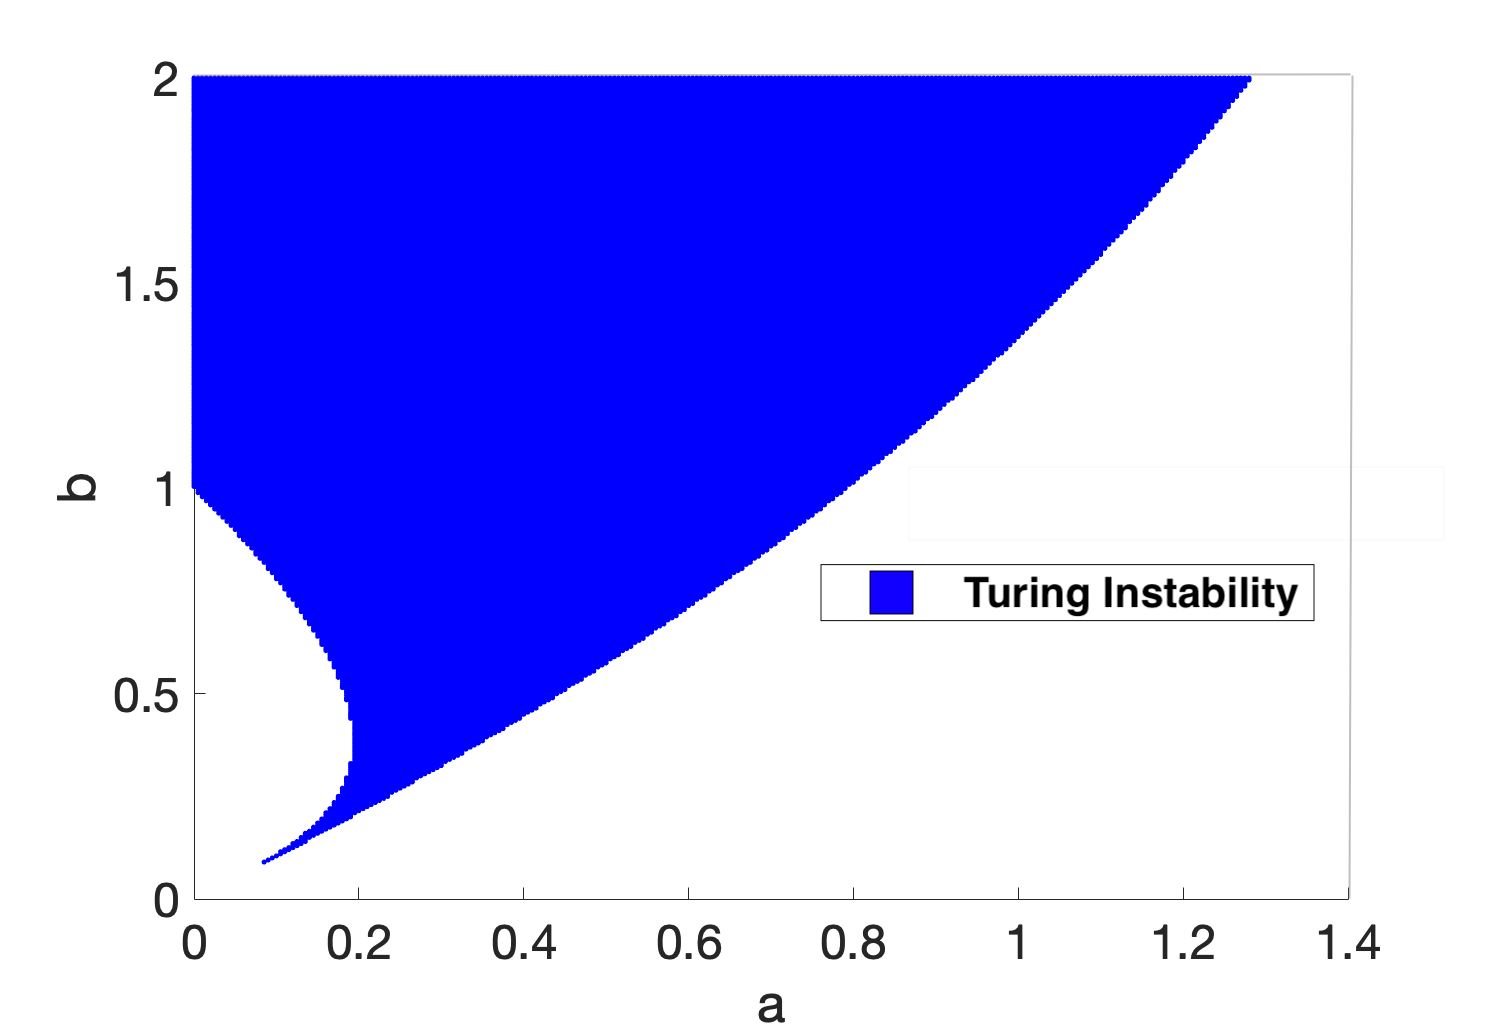
\includegraphics[width=7cm,height = 6cm]{turingspace.png}
        \caption{Turing space, no delay. $\epsilon^2=0.001$.}
        \label{fig:turingspace}
    \end{subfigure}
    \caption{Conditions \eqref{cond1} and \eqref{cond2} used to plot bifurcation diagram and Turing space for parameters $(a,b)\in[0,1.4]\times[0,2]$, for the Schnakenberg model.}
    \label{fig:dispfixed}
\end{figure}

\subsection{Numerical Implementation}\label{section:numimp}
In order to numerically resolve the spatial derivatives $\frac{\partial^2 u}{\partial x^2}$, $\frac{\partial^2 v}{\partial x^2}$ and implement the relevant boundary conditions, a finite-difference scheme is used. Throughout the dissertation we use $m=500$ equally spaced spatial discretisation points on the domain $x\in\Omega=[0,1]$. This discretisation results in $m=500$ \tb{ODEs} or DDEs in time, which are solved \tb{via built-in timestepping solvers in Julia}. Further details on the derivation and implementation of the finite difference scheme and boundary conditions can be found in Appendix \ref{section:appA}.

Reaction-diffusion systems can be numerically stiff to solve \cite{stiff1, william}, and thus to solve these systems with time delay, we require stiff numerical solvers suitable for DDEs. The inherent stiffness of the problem makes standard DDE solvers in MATLAB such as \emph{dde23} and \emph{ddesd} unsuitable, and past work has been restricted in the progress made through numerical simulations \cite{william} due to the computationally expensive task of solving reaction-diffusion systems with non-stiff solvers. Standard stiff solvers in MATLAB, such as \emph{ode23s} and \emph{ode15s} do not support time delay. For this dissertation we therefore develop neat and efficient code using the Julia language to numerically solve these systems. Julia has an extensive differential equations solver suite \cite{rodas}, and has the capability to apply the method of steps \cite{methsteps} to a stiff solver, allowing the incorporation of fixed time delays. Throughout the dissertation we use absolute and relative solver tolerances of $10^{-6}$, with a maximum timestep set as $0.1$. For these tolerances, the default stiff solver implemented by Julia is \emph{Rodas5}, a 5-th order A-stable solver, from the family of Rosenbrock methods \cite{rodas}. An interested reader can find more details on Rosenbrock methods in \cite{rosenbrock}. The Julia code used to generate all numerical solutions throughout this dissertation can be found at \cite{git}.

Finally, since the Schnakenberg model has \textit{cross} reaction kinetics, as discussed in Section \ref{section:background}, we have that when the concentration of the activator $u$ is high, the concentration of the inhibitor $v$ is low, and vise-versa \cite{murray}. The concentration gradients of the two morphogens $u$ and $v$ are thus effectively `out of phase', and so it is sufficient to consider just the numerical solution of the activator $u$. Throughout the dissertation therefore, where relevant, only the numerical solution of the activator $u$ is plotted.
